\section{Experimental Platform}
\label{sec:platform}

\begin{figure*}[htb]
     \centering
         \centering
         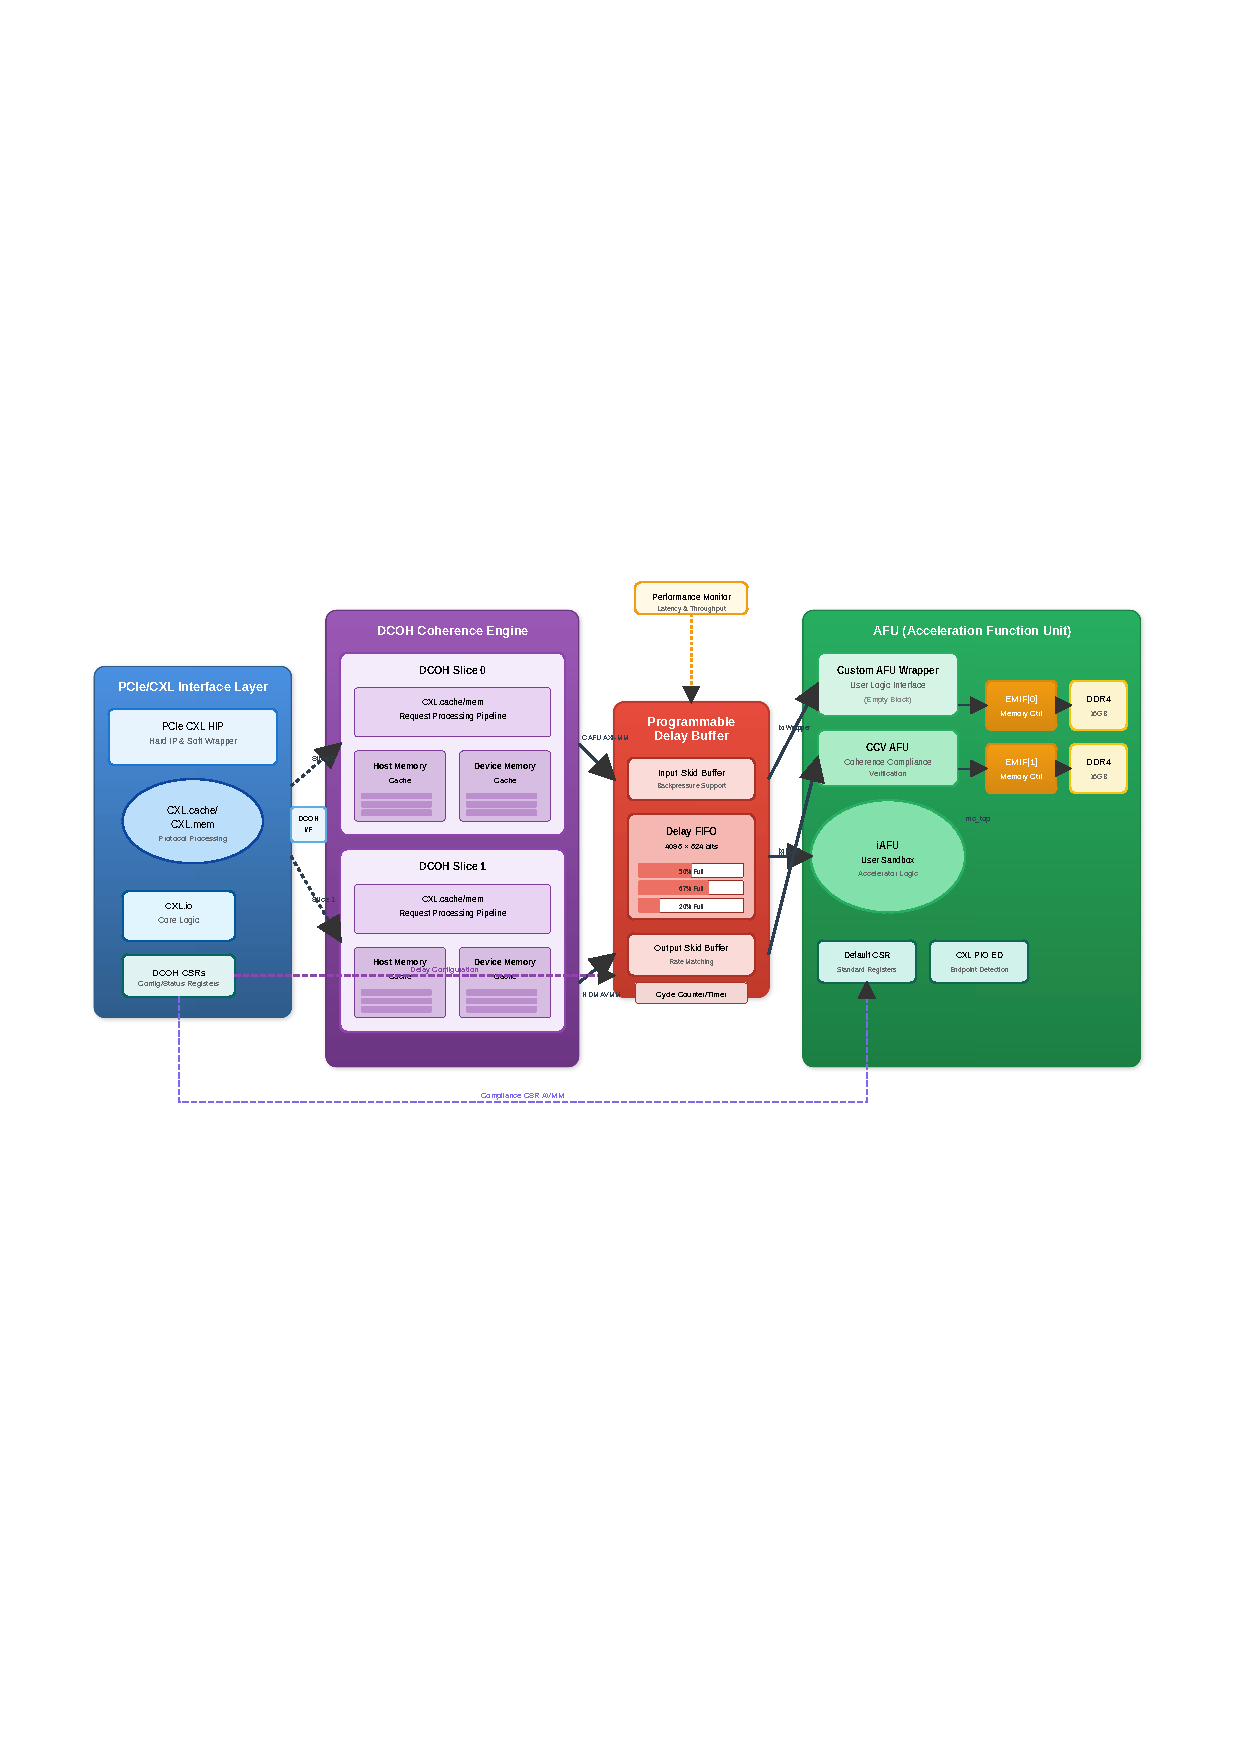
\includegraphics[width=\linewidth]{figures/cxl-fpga-architecture.pdf}
         \caption{CXL Type-2 FPGA platform architecture with programmable delay buffer. The delay buffer intercepts read responses between the CXL controller and memory controller, injecting configurable latency to emulate different CXL fabric topologies. Write operations bypass the delay buffer as lock implementations are dominated by read-path latency from polling.}
         \label{fig-cxl-fpga-arch}

\end{figure*}

Evaluating synchronization across CXL access modes requires a platform that supports both hardware-managed and software-managed coherence with controllable memory latency.
No commercially available CXL device provides all of these capabilities: existing CXL memory expanders (Type~3) lack hardware coherence, while CXL switches with multi-host support are not yet available with programmable latency control.
We therefore build an FPGA-based CXL Type-2 device that provides these capabilities.

\paragraph{Scope of the platform.}
Our platform emulates a \emph{single-host} CXL environment where one host accesses device-attached memory through the CXL.mem and CXL.cache protocols.
We do not emulate multi-host switched topologies; instead, we use multiple threads on a single host to study the coherence protocol behavior that would occur between concurrent accessors.
While this does not capture cross-host network effects (e.g., switch hop latency, inter-host snoop forwarding), it isolates the coherence protocol overhead from network effects, which is our primary measurement goal.
We discuss the limitations of this single-host setup in Section~\ref{sec:discussion}.

\subsection{Hardware Configuration}

The platform is built on a BittWare IA-780i accelerator card with an Intel Agilex~7 FPGA and Intel CXL IP core.
The card connects to the host via PCIe~5.0~x16 and exposes 32\,GB of on-board DDR4 as CXL-attached memory.
The host is a Xeon~6 Granite Rapids 6787P with 256\,GB DDR5 MRDIMM, running Linux 6.x with CXL driver support.

The FPGA is configured as a CXL Type-2 device supporting both CXL.mem (for memory access) and CXL.cache (for hardware coherence via BISnp).
This configuration allows us to test all four access modes described in Section~\ref{sec:access-modes}:
\begin{itemize}
    \item \textbf{Cached-HC:} CXL.cache active, BISnp manages cache-line ownership. RMW atomics available.
    \item \textbf{Cached-SC:} CXL.cache disabled, software manages consistency via fences/flushes.
    \item \textbf{UC:} Host page table entries marked uncacheable via PAT; loads/stores bypass host cache, go directly through CXL.mem.
    \item \textbf{NT:} Non-temporal instructions (\texttt{movntdq}/\texttt{movntdqa}) bypass cache; stores exploit write-combining buffers.
\end{itemize}

\subsection{BISnp Coherence Implementation}

Our FPGA implements the BISnp protocol for hardware-managed coherence using an inclusive snoop filter.
The snoop filter tracks cache-line ownership using a set-associative structure (4096 sets, 8-way associative) stored in FPGA BRAM.
Each entry records the cache-line address (tag), the owning host, and the coherence state (Invalid, Shared, Exclusive, Modified).

When the host issues a load to a line not present in the snoop filter, the device allocates a new entry in Shared state.
When the host issues a store or RMW atomic, the device must transition the line to Exclusive/Modified state.
If another entry already holds the line (possible in a multi-host scenario; in our single-host setup, this occurs when a different thread's access pattern has invalidated the prior owner's copy), the device issues a back-invalidation to force writeback before granting exclusive access.

The snoop filter lookup adds 2--4 cycles (5--10\,ns at 400\,MHz) to every memory access under Cached-HC mode.
This overhead is absent under Cached-SC, UC, and NT modes, where the snoop filter is bypassed entirely.
This per-access overhead is small in isolation but accumulates significantly under high-contention polling, where a lock variable may be read hundreds of thousands of times per second by each thread.

\subsection{Access Mode Implementation}

Switching between access modes requires coordinated changes at the host and device levels:

\paragraph{Cached-HC.}
The default configuration.
CXL memory is mapped with writeback (WB) cacheability via the host page table.
The FPGA's CXL.cache interface is active, and the snoop filter tracks all cache-line accesses.

\paragraph{Cached-SC.}
CXL.cache is disabled in the FPGA configuration; the snoop filter is inactive.
Host-side mapping remains WB cacheable, but the benchmark explicitly inserts \texttt{clflush} after stores and \texttt{lfence} before loads to shared lock variables to ensure visibility.

\paragraph{UC.}
The host maps CXL memory pages with the UC (uncacheable) memory type via the PAT (Page Attribute Table).
All loads and stores bypass the host cache hierarchy and are issued directly as CXL.mem transactions.
The FPGA processes these as simple memory reads/writes without snoop filter involvement.

\paragraph{NT.}
The host maps CXL memory with the WC (write-combining) memory type.
Stores use \texttt{movntdq} (128-bit non-temporal store) and are coalesced in the host's WC buffers before being flushed to the device.
Loads use \texttt{movntdqa} (128-bit non-temporal load) to avoid cache pollution.
An \texttt{sfence} after each store ensures the WC buffer is flushed and the store is globally visible.

\subsection{Programmable Delay Injection}

To emulate different deployment latencies, we implement a delay buffer in the FPGA fabric between the CXL controller and the DDR4 memory controller.
The buffer intercepts read responses and holds them in a 4096-entry FIFO until a target release cycle, computed as the enqueue timestamp plus the programmed delay value.
The delay is configurable from 50\,ns to 10\,$\mu$s with 10\,ns granularity via a memory-mapped register at PCIe extended capability offset \texttt{0xE08}.
Read and write delays are independently configurable.

The implementation employs a 12-bit free-running cycle counter at 400\,MHz for timestamp-based release.
Modular arithmetic handles counter wraparound correctly.
Input and output skid buffers maintain AXI4 protocol compliance and provide elastic flow control, achieving single-cycle throughput for enqueue and dequeue operations in the common case.
The 524-bit internal data path accommodates the full 512-bit payload plus 12 bits of metadata (transaction ID, response status, last-beat indicator).

We test four latency configurations:
\begin{itemize}
    \item \textbf{DRAM baseline:} No injected delay (local DDR4 latency only, approximately 80\,ns).
    \item \textbf{400\,ns:} Representative of CXL memory within the same chassis. This aligns with measured latencies on real CXL switches (340--650\,ns range reported in recent measurements~\cite{yangUnlockingPotentialCXL2025}).
    \item \textbf{2\,$\mu$s:} Represents multi-hop CXL fabric scenarios with switch traversal overhead. While extreme, this latency enables us to study asymptotic behavior and identify trends.
    \item \textbf{10\,$\mu$s:} Represents extreme multi-hop CXL fabric scenarios or congested switch paths. This configuration stress-tests lock implementations at latencies where per-access costs dominate, exposing whether algorithmic efficiency (e.g., $O(\log N)$ vs.\ $O(N)$ polling) or access mode choice has a larger impact on throughput.
\end{itemize}

\paragraph{Validation.}
We validate delay accuracy by measuring round-trip latency using a pointer-chasing microbenchmark (sequential dependent loads) and comparing against the programmed delay value.
Measured latencies are within 3\% of programmed values across the entire range, with the residual attributable to DDR4 access latency and AXI protocol overhead.

\subsection{Resource Utilization}

The complete implementation---including delay buffer, snoop filter, skid buffers, and debug infrastructure---consumes approximately 8\% of FPGA LUT resources and 15\% of BRAM per memory channel, achieving timing closure at 400\,MHz.
For our eight-channel configuration, total BRAM utilization is approximately 35\%.
Performance counters track transaction counts, buffer occupancy, and back-pressure events for experimental validation.
